%\section{Mathematical Modeling}
\label{sec:mathmodel}

% \begin{itemize}
% \item \st{unstable stratified boundary layers (raleigh number estimate)}
% \item \st{justify incompressible N-S}
% \item \st{justification of far-field eddy-viscosity model (M-O)}
% \item modeling eddy-viscosity in device 
% \item vane and turbine representation via penalty function // immersed boundary method
% \item cone representation
% \end{itemize}

%remember that \st{} is strikethrough
%
% should this all be math modeling?
%

The aim of this work is to simulate synthetic
dust devils in the field. This requires a model of the ambient
conditions for a representative case, such as Arizona, where
experimental data is available from tests that have been
performed. Furthermore, for this to be generally useful in the
prediction of flows in a variety of conditions, we need a model
applicable to any flow near the surface of the earth.  

This chapter details an analysis of surface fluid mechanics, and
develops a mathematical model for turbulence in a thermally stratified
medium. We seek to emulate the operation of the apparatus during the
day, when dust devils are observed to form readily. 
At these times, the atmospheric surface layer has the following
character. Incident radiation from the Sun does not significantly
interact with the air, which is nearly transparent. Instead, this
radiation is absorbed by the ground, which causes its temperature to
rise. This results in a thermal gradient between the hot ground and the
cooler air. The warm ground conducts heat to the air, causing expansion
and lowering the density of the air. This reduced density air near the
surface is driven upwards by the force of buoyancy.  

For sufficiently large temperature gradients, the hot surface layer is
unstable, and as the warm air is driven upwards the flow will transition
to turbulence. For the typical use case we consider, namely Arizona in
summer, the temperature difference can be in excess of 30 Kelvin. 
Rayleigh numbers associated with temperature gradients of this magnitude
are between $10^{9} - 10^{11}$ and therefore meet the criterion
% ref thermo book here?
for transition to a turbulent regime. The flow is that of an unstably
stratified fluid.  

This chapter begins by describing the governing equations of the system
of interest. It then proceeds to the development of a viscosity model
used to resolve the large scale features of the solution. Next, models
used to represent the vanes and turbine, and the separation of
fluid off of these modeled surfaces, are introduced.  Finally, the
models for the computational domain extent and the boundary conditions
are discussed. 

%Note that a complete numerical specification of all the model
%parameters introduced in this chapter are provided in a table in
%appendix \ref{app:model_param}.

\section{The Governing Equations of Fluid Motion}
\label{sub_sec:ns_en}
%
% do I need to justify this more? These are pretty critical, after all
%

The equations describing fluid flow with natural convection are,
\begin{align}
  \frac{\partial u}{\partial t} + u \cdot \nabla u =& \,
  -\frac{1}{\rho}\nabla P + \nu \nabla^2 u - g \frac{T'}{T_0}\\
  \nabla \cdot u =& \, 0 \\
  \rho c_p \frac{\partial T}{\partial t} + u \cdot \nabla T =& \, \nabla
 \cdot ( k \nabla T)
\end{align} 
under the assumption that the temperature variation is small in
comparison to the mean temperature of the region. These are the
incompressible Navier-Stokes equations with Boussinesq, a representation
of buoyancy coupled with the heat equation.  
%
% in full document be sure to mention that neglecting coriolis is legit
% below 50ms
%
%
As discussed above, we anticipate that the flow will be
turbulent. Turbulence significantly alters the character of the flow,
and necessitates either resolving the resulting small scales or
providing a model that emulates their impact. In this case, a
Reynolds Averaged Navier-Stokes (RANS) formulation is used, where the 
turbulent viscosity and thermal conductivities are permitted to vary in
space, and the flow is decomposed into constant laminar and varying
turbulent and vane components,  

\begin{eqnarray*}
 \nu =& \nu_{l} + \nu_{T}(z) + \nu_{V}(r,z) \\
 K =& K_{l} + K_{T}(z) + K_{V}(r,z).
\end{eqnarray*}

This is an effective eddy viscosity model, and the subsequent two
sections will elaborate on the spatial dependence and character of
$\nu_T$, $K_T$, $\nu_C$ and $K_C$. The laminar, base diffusivities 
are $\nu_l$ and $K_l$, which do not vary in space. 

\section{Viscosity Model}

We use the well-known similarity model of Monin and
Obukhov\cite{monin2007statistical,monin1954basic,1990JFM...212..637K} as
a guide to the specification of an eddy viscosity model to describe the
vertical mixing in the atmosphere. This formulation is an extension of
the mixing-length model of Prandtl, where the concepts of gradient
diffusion and mixing length were generalized to thermally stratified
flow.    

%ADD DIMENSIONS TO MAKE SCALING MORE CLEAR\todo{add dimensions}
%
% justify prandtl assumption here
%

Monin and Obukhov argued that under statistically stationary, horizontally
homogeneous conditions, the dynamics of any mean turbulent quantity
($\bar f$) in a thermally stratified medium depend only on,  

\begin{equation}
\bar f = f(z,\frac{g}{T_0},\rho_0,\nu_l,K_l,u^*,q).
\end{equation}
Aside from near the surface, the laminar diffusivities $\nu_l$ 
and $K_l$ will be  
small compared to their turbulent counterparts, $\nu_T$ and $K_T$, and 
are therefore negligible. 
The remaining five parameters are: the distance from the ground, z; the
buoyancy coefficient, $\frac{g}{T_0}$; the density of the fluid,
$\rho_0$; a velocity scale, $u^*$ (in particular, the freestream
velocity); and the heat flux to the ground, $q$. %\todo{is this right?}
% Likewise, if we define $z-z_0$ as an ``effective roughness
% height'' or displacement distance, we can reasonably neglect $z_0$ from these
% considerations. While the roughness height can be large (for instance in
% a cornfield, where the roughness height could reasonably be several
% meters), for the present study the expectation is that this roughness
% height will be on the order of centimeters\cite{oke1987boundary}, and
% therefore negligible.  
%
% add refence to dynamical and physical meteorology 
% 
These primary quantities have the following dimensions,

\begin{eqnarray}
 \textbf{Height:}& z\enskip \dot = \enskip [m]  \\
 \textbf{Buoyancy:}& \qquad \frac{g}{T_0}\enskip \dot = \enskip [kg] [m] [s]^{-2}
  [K]^{-1} \\ 
 \textbf{Density:}&  \enskip \rho \enskip \dot = \enskip [kg] [m]^{-3}  \\
 \textbf{Velocity:}& \enskip u^* \enskip \dot = \enskip [m] [s]^{-1} \\
 \textbf{Heat Flux:}& \enskip q \enskip \dot = \enskip [kg] [s]^{-3} 
 %\textbf{Height:}& z \rightarrow \text{Units}: Meters \rightarrow [m]  \\
 %\textbf{Buoyancy:}& \frac{g}{T_0} \rightarrow Units: Meters \rightarrow
 % [m]  \\ 
 %\textbf{Density:}& \rho \rightarrow Units:  \rightarrow
 % [m]  \\ 
 %b & b
\end{eqnarray}

Our unknown mean turbulent quantity ($\bar f$) depends on four
dimensions: length, time, temperature and mass. Dimensional analysis
implies that this should then only be a function of a single dimensionless
group\cite{munson2012fundamentals}. This is chosen to be,
\begin{equation}
 \xi = -\frac{\kappa \frac{g}{T_0} \frac{q}{c_p \rho_0} z}{ {u^*}^3}.
\end{equation}
where $\kappa$ is the (dimensionless) Von-Karman constant. 
The physical meaning of this quantity bears some discussion.  
The numerator, $\kappa \frac{g}{T_0} \frac{q}{c_p \rho_0} $, is
proportional to the buoyant production of kinetic energy.  The
denominator, $\frac{{u^*}^3}{z}$, is a shear production rate. 

The non-dimensional group $\xi$ is typically cast into the following 
form, 
\begin{equation}
 \xi = \frac{z}{L_{M-O}}
\end{equation}
where $L_{M-O}$ is the famous, ``Monin-Obukhov'' length,
\begin{equation}
 L_{M-O} = -\frac{{u^*}^3}{\kappa \frac{g}{T_0} \frac{q}{c_p \rho_0}}. 
  \label{eqn_mo_length}
\end{equation}

This length can be interpreted as the vertical location
where the production of buoyantly generated kinetic energy is
approximately equal to the energy generated by wind shear. When the
magnitude of $L_{M-O}$ is large, the flow is dominated by shear effects,
and the impact of buoyancy is small. Conversely, a small magnitude of
$L_{M-O}$ implies that buoyant effects largely dominate the kinetic
energy production. Notice also that the sign convention in Equation
\ref{eqn_mo_length} is such that for the systems we consider (q>0, heat
flux from the surface to the air), $L_{M-O}$ will always be
negative. This is as expected, as the convection from the high
temperature surface to cooler air is unstable. 

%The mean quantity $\bar f$ has a
%functional representation to the effect,
In this case, appropriately normalized mean turbulent quantities should
be functions of only the non-dimensional group 
\begin{equation}
 \frac{\bar f}{f_{MO}} = \phi(\frac{z}{L_{M-O}})
\end{equation}
with $f_{MO}$ a normalizing constant with units of $\bar f$, and $\phi$
is a function only of $\xi$. We are interested in the case where
$\xi<0$, which corresponds to heat flux from the ground into the
air. For instance, the mean velocity field would have scaling,
$\frac{u^*}{\kappa}$ and the temperature fields would be scaled as $T^*
= \frac{1}{\kappa u^*} \frac{q}{c_p \rho_0}$. In this way, the mean
velocity and temperature fields would have the form,  
\begin{eqnarray}
\bar u(z) = \frac{u^*}{\kappa} \phi_u(\frac{z}{L_{M-O}}) \\
\bar T(z) = T^* \phi_T(\frac{z}{L_{M-O}}).
\end{eqnarray}
As a result, the vertical gradients of the velocity and temperature are
necessarily, 
\begin{eqnarray}
\frac{\partial \bar u(z)}{\partial z} = \frac{u^*}{\kappa L_{M-O}}
 \varphi_u(\frac{z}{L_{M-O}}) \label{eq:uz} \\ 
\frac{\partial \bar T(z)}{\partial z} = \frac{T^*}{L_{M-O}}
 \varphi_T(\frac{z}{L_{M-O}}) \label{eq:tz}.
\end{eqnarray}
Notice that $\phi$ and $\varphi$ are different universal functions. Eddy
viscosity is defined as, $u'v' = \nu_T \frac{\partial
u}{\partial z}$\cite{durbin2001statistical}, in which case, using
equation \ref{eq:uz}, it must scale as
\begin{equation}
 \nu_T = \frac{{u^*}^2}{\frac{\partial \bar u}{\partial z}} = \frac{u^*
  \kappa L_{M-O}}{\varphi_u(\xi)}.
\end{equation}
While eddy thermal diffusivity (defined as, $q = c_p \rho_0 K_T
\frac{\partial T}{\partial z}$) is 
\begin{equation}
 K_T = \frac{q/c_p \rho_0}{\frac{\partial \bar T}{\partial z}} = \frac{u^*
  \kappa L_{M-O}}{\varphi_T(\xi)}.
\label{eqn:eddy_kt}
\end{equation}
Note the difference between $\varphi_u$ and
$\varphi_T$, which for turbulent Prandtl numbers near unity (e.g. $Pr_T
\approx 1$) the functions will be identical. The asymptotic behavior of
the $\varphi_T$ and $\varphi_u$ at large and small values of $\xi$
provides guidance to the more general character of the functions. 
Our interest lies in the case where $L_{M-O}<0$, which corresponds to heat flux
from the ground into the air.  
%


The case where $\xi \to -\infty $ implies $\frac{z}{L_{M-O}} \to
-\infty $ and $z>>L_{M-O}$. This is most readily interpreted as the instance
where $u^* \to 0$, e.g. the buoyancy-dominated case with no wind
(free-convection). For this case, the function $\varphi_T$ must have no
dependence on $u^*$, and will approach a constant. Scaling
analysis implies that the overall function will not depend on $u^*$ only
when the function $\varphi$ scales to the $-\frac{4}{3}$ power. The
function must then be

\begin{equation}
 K_T = \frac{1}{C_T} \left( \frac{q}{c_p \rho_0} \frac{g}{T_0}
		     \right)^\frac{1}{3} z^{\frac{4}{3}}  \text{ 
for } z \gg L_{M-O}. 
\end{equation}

So long as the Prandtl number remains constant in space, then
% todo: provide discussion as to why this is not an unreasonable expectation
identical arguments regarding the asymptotic behaviour at large $\xi$ provide
the analogous result for the eddy viscosity's variation with respect to
distance from the ground,  
\begin{equation}
 \nu_T = \frac{1}{C_{\nu_T}} \left( \frac{q}{c_p \rho_0} \frac{g}{T_0}
			     \right)^\frac{1}{3} z^{\frac{4}{3}}  \text{ 
for } z \gg L_{M-O}. 
\end{equation}

\subsection{Shortcomings of Monin-Obukhov Theory}

Several known (and often well characterized) shortcomings of the Monin
Obukhov similarity theory exist. These include:

\begin{itemize}
 \item Surfaces with large spatial variations in roughness heights
 \item Outside of the surface layer (several hundred meters) where the 
       coriolis effect is no longer negligible
%\item the theory's predictions are well known to be sensitive to choice
%      of universal function for $L>0$.
\end{itemize}

In ``ideal'' situations, the theory has been found to be
accurate to more than 10\%\cite{QJ:QJ49709741204,kaimal}. 
For our case, with minimal surface roughness and our interest
constrained to the near surface layer, these functions are applicable
and reasonably accurate\cite{Foken2006}, and are easily implemented in
software.  

\section{Eddy Viscosity in the Device}

%However, this is also a more
%difficult regime to model.\todo{poor justification} 
The validation process identified a refinement to the virtual vane
formulation that results in a better representation of the vane
effects in a broader range of flows. The thermal and momentum
diffusivities are even larger in the device where the flow across the
vanes produces shear and generates turbulence. The model now include an
enhanced turbulent diffusivity in the vortical plume region to account
for the effects of vortex shedding from the trailing edge of the vanes,
which is not represented in the virtual vane representation (discussed in
\ref{subsec:vane}). 

% To successfully accomplish this, source terms
% for production of diffusivity were formulated to properly
% account for the generation of turbulence in the region of the
% vanes. This diffusivity would then convect and diffuse through space. 
% To avoid modeling a temporal and three-dimensionally spatially
% varying field of diffusivities, we have instead calibrated the field
% based on data provided by our partners at Georgia Tech. 

%This calibration
%is detailed in Section \ref{sec:validation}. 
The eddy-viscosity in the region of the vanes and interior is set based
on scaling relations for a turbulent self-similar circular jet, as
described in Pope\cite{pope2000turbulent},
 
\begin{equation}
  \nu_C = U_0 y_{1/2} \bar \nu_C.
  %\nu_C(r) = U_0(r) y_{1/2}(r) \bar \nu_C
\end{equation}

In this equation, $U_0$ is the peak velocity, and $y_{1/2}$ the jet
half-width (taken to be the dust devil half-width).  
% In words, we are scaling the
% calibrated viscosity by the velocity and length scale of the
% apparatus. $\bar \nu_C $ is input, measured from the experimental
% laboratory.  The diffusivity here is essentially a top hat filter, which
% radial values interior to the vanes the nominal calibrated value, and
% those outside the vanes zero, e.g. $\nu_C(r>r_{\text{vane}})=0$. 
The dimensionless constant $\bar \nu_C $ is calibrated based on
experimental data, and is set to zero outside the device. 
The thermal diffusivity inside the device, $K_C$, is then fixed with the 
assumption that the Prandtl number is unity.  

%The thermal and momentum diffusivities are expected to be even larger in the
%device where the flow across the vanes produces shear and generates
%turbulence. Our model for the diffusivities inside the vanes should
%therefore be higher than the ambient regions outside the vanes. 



\section{Vane Representation}
\label{subsec:vane}
To rapidly prototype general system configurations, the
computations must be able to explore a large space of possible
geometries and settings. This presents a significant meshing and 
computational challenge if the detailed flow around the vanes is to be
computed. In the region near the vanes, where a no-slip boundary
condition is imposed, the flow will necessarily form a thin momentum
boundary layer. Resolving this boundary layer requires high resolutions
immediately adjacent to the walls. Changing the vane location requires
that a new mesh be generated. This is a significant
challenge, as the development of a new mesh often requires significant
human effort and time. Furthermore, the process is error-prone, 
and would require that each simulation using a new mesh undergo 
detailed solution verification. 


% Your text on the virtual vanes does not provide enough information to
% know exactly what we did. It is needlessly vague, and does not
% adequately connect to the real vane geometry. I propose the following
% more direct and more precise text. Further, the penalty nomenclature
% is inappropriate.

Instead, we have developed a modeling formulation that does not require
explicitly meshing the turning vanes, or any surface. These so-called
``virtual vanes'' are implemented as a body force that 
is applied in the annular region that contains the vanes. 

   \begin{figure}[!htb]
    \centering
    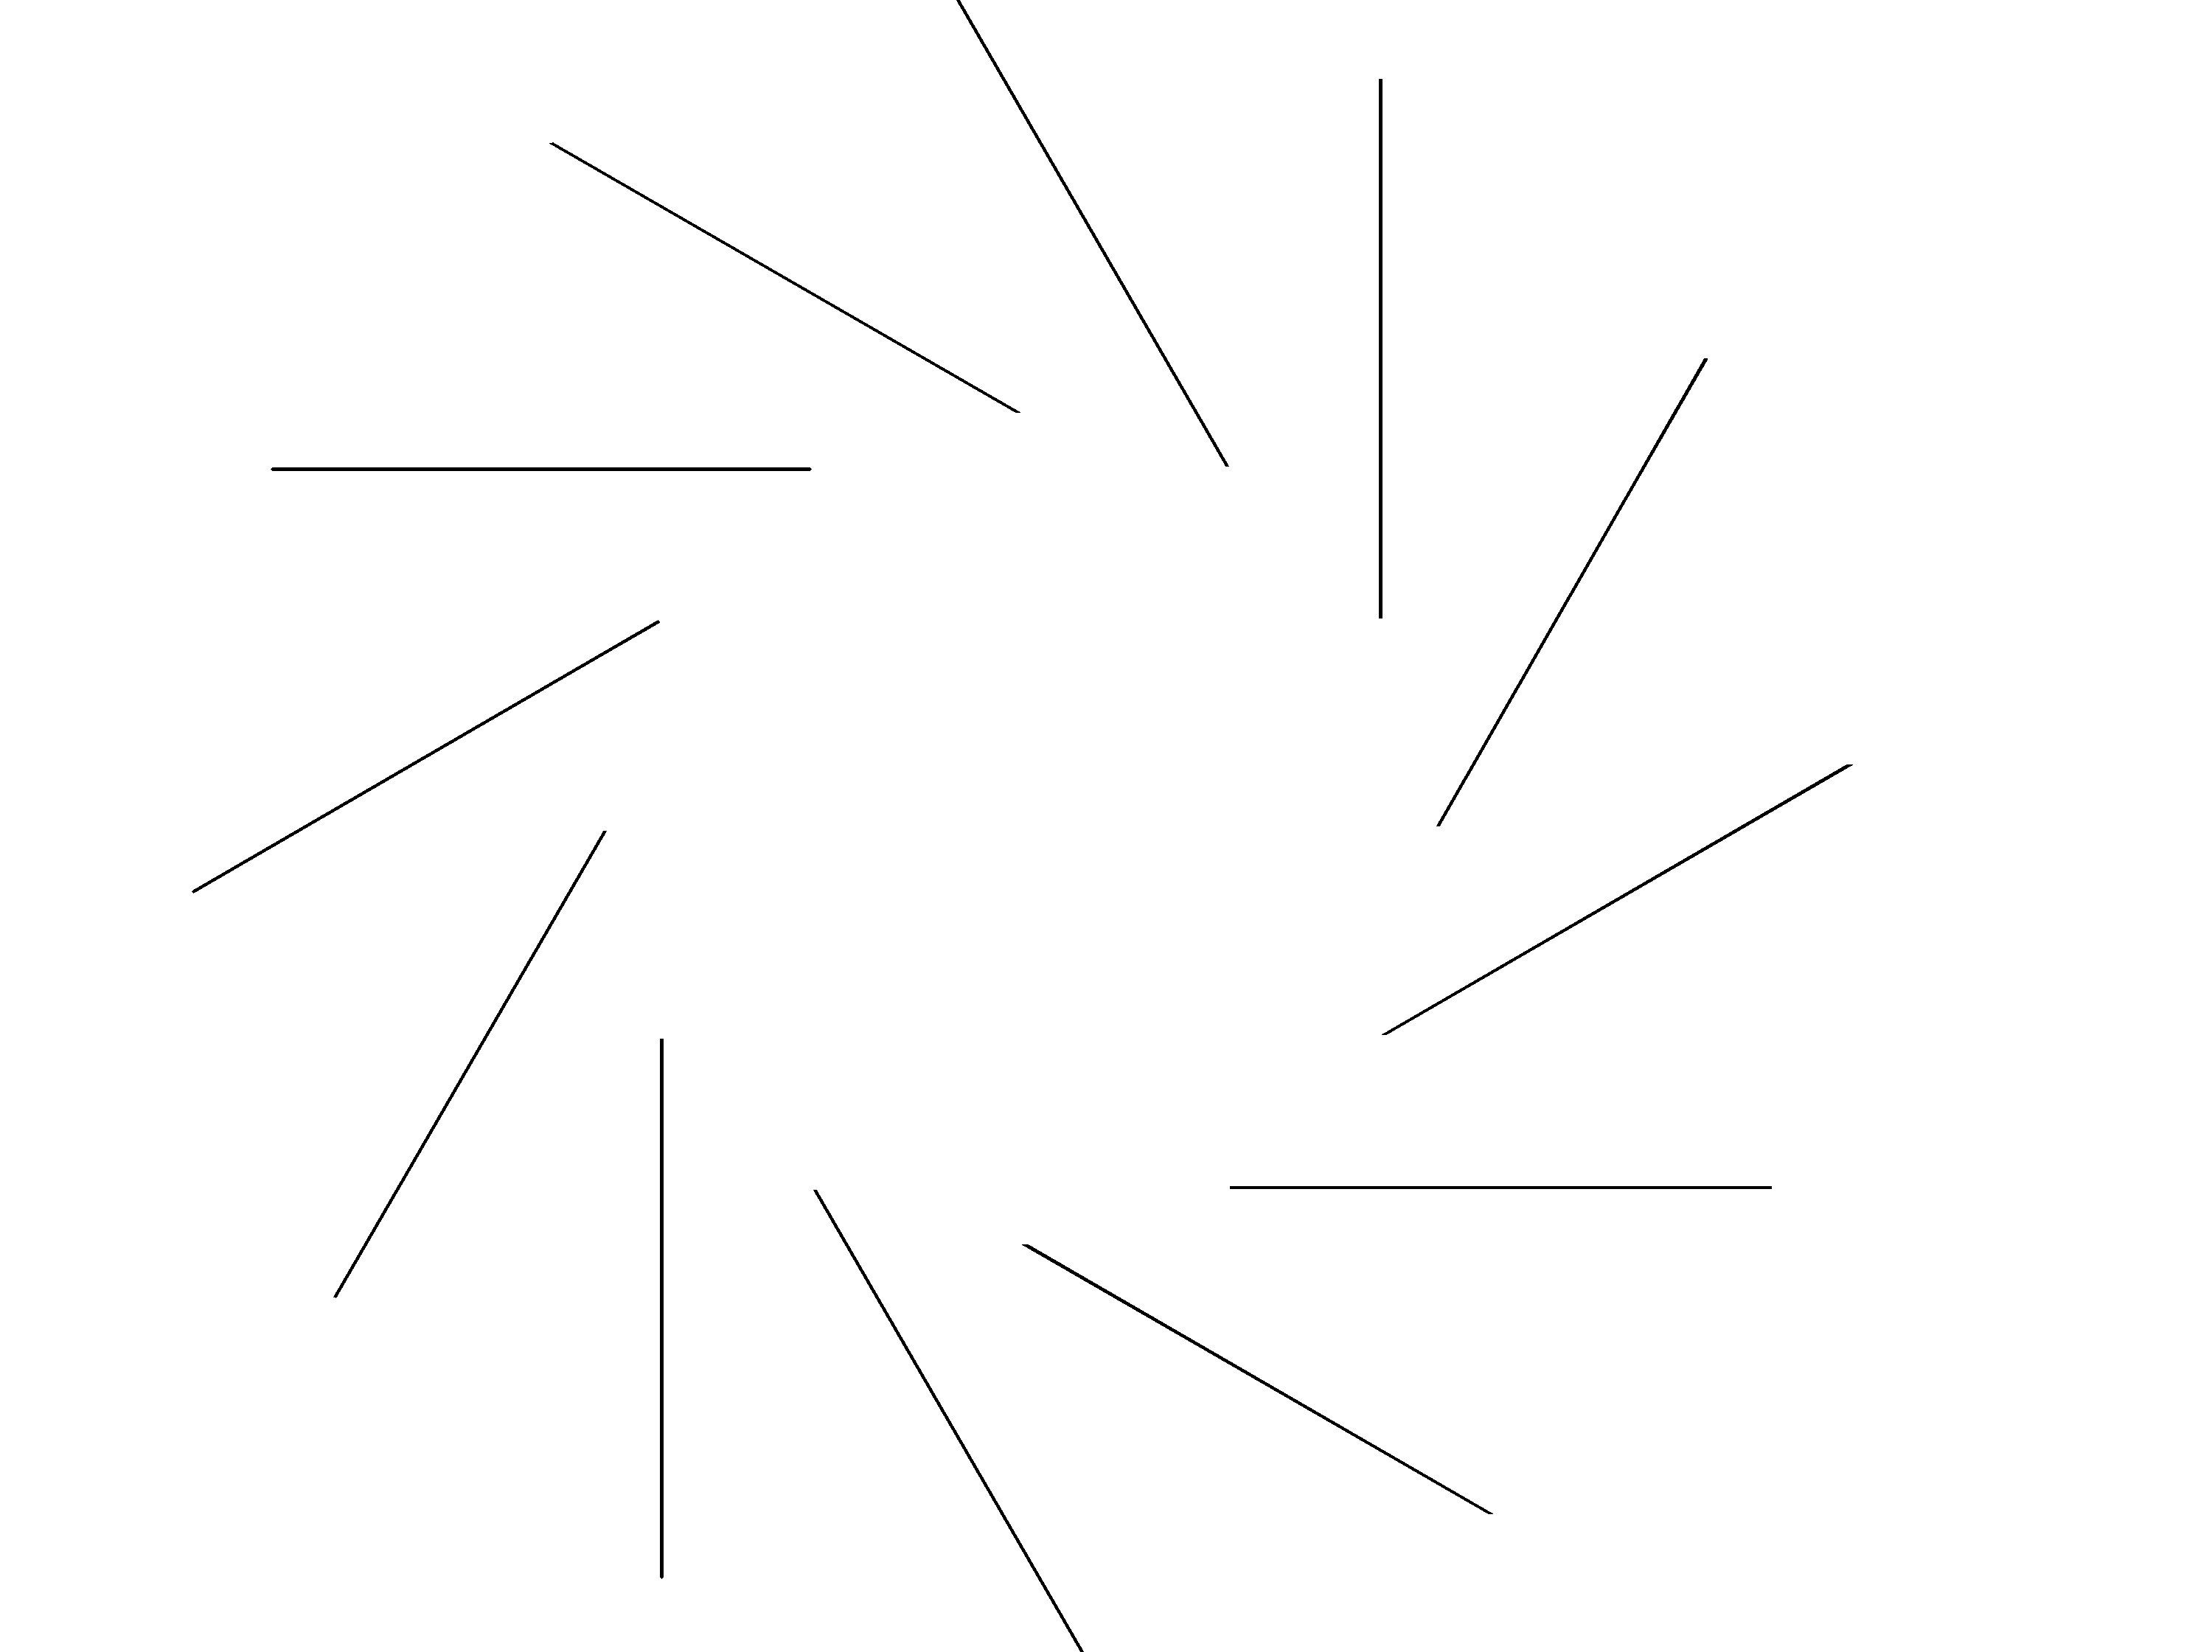
\includegraphics[width =0.47\textwidth]{figs/gridded_region}
    \hfill
    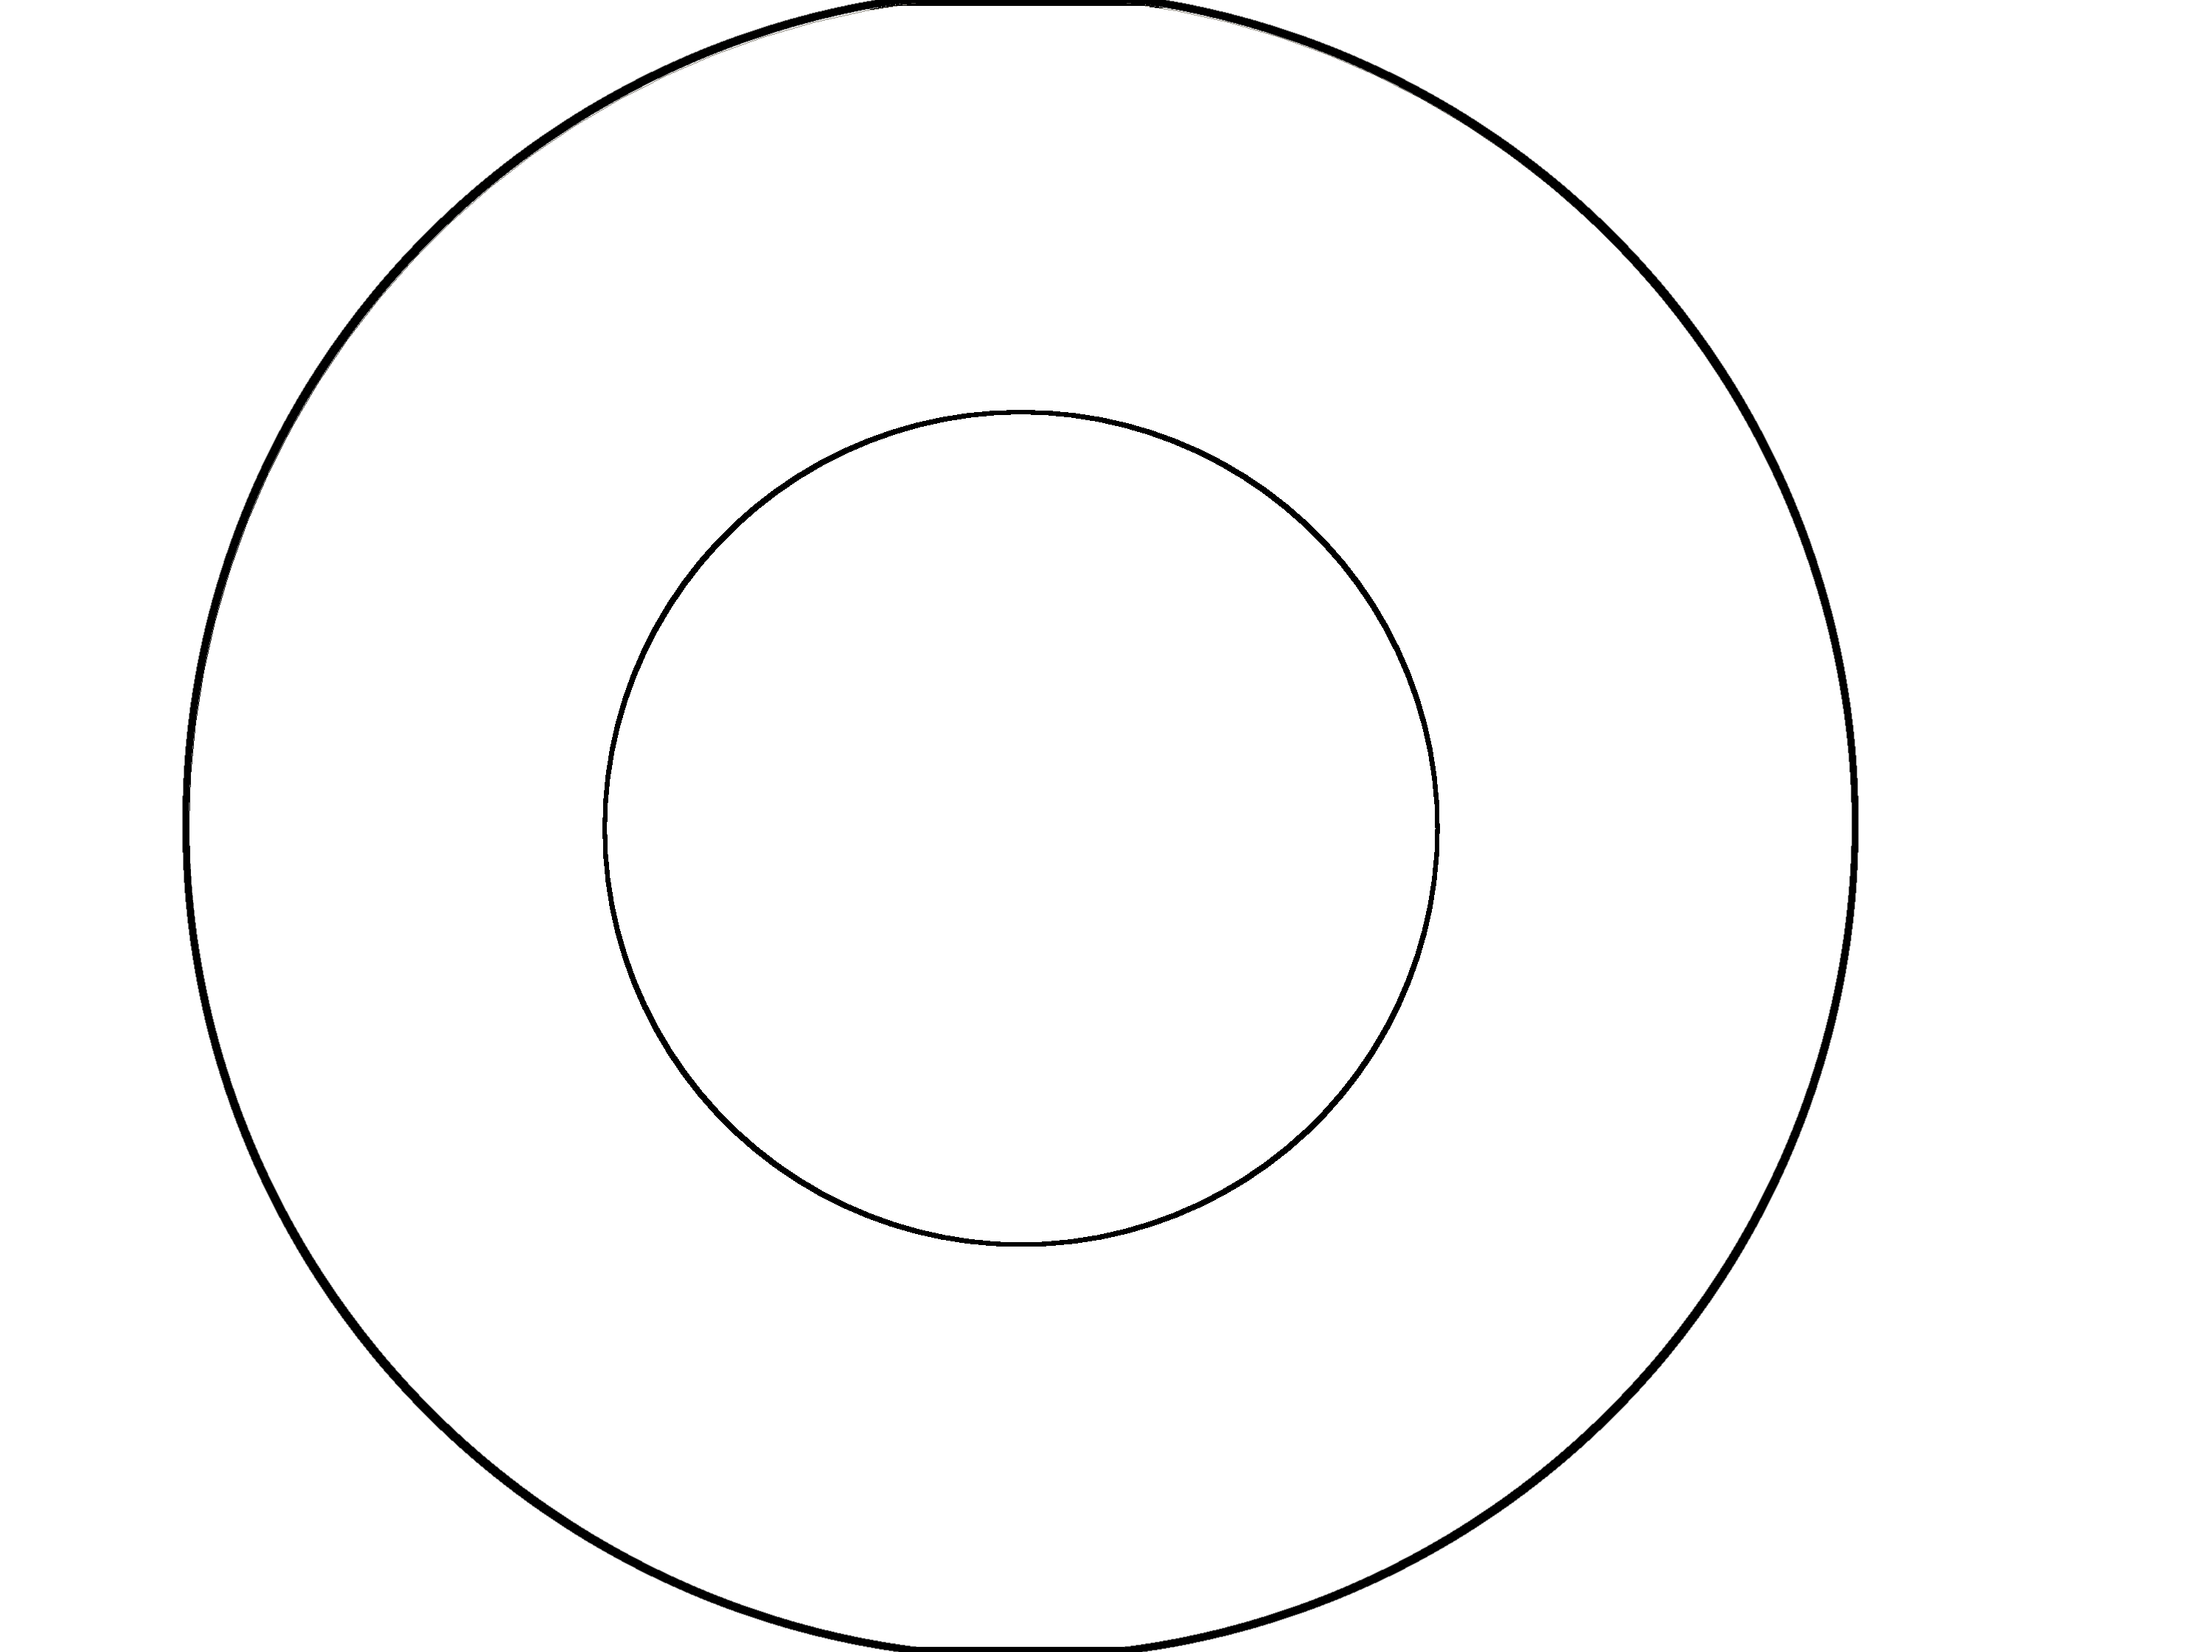
\includegraphics[width =0.47\textwidth]{figs/forcing_region}
     \caption{An example of explicitly represented turning vanes (left)
    versus an annular forcing region (right).}
     \label{fig:penalty_model}
   \end{figure}



Vane geometry is specified by the angle $\phi$ a vane makes with a
radial line as a function of the radial coordinate, $r$, and the polar
angle, $\theta$. A unit normal to the vane surface ${\bf n}$ is defined
as 
%
\begin{equation}
 {\bf n}({\bf x}) = \sin \left(\phi(r,\theta) \right) \hat{{\bf r}}+ \cos
  \left(\phi(r,\theta) \right) \hat{{\bf \theta}} 
\end{equation}
%
where $\hat{{\bf r}}$ and $\hat{{\bf \theta}}$ are unit
vectors in the radial and azimuthal directions, respectively.
With this vane-normal vector field specified, a body force ${\bf f_v}$
is defined
that will drive the velocity in the ${\bf n}$ direction toward zero,
effectively turning the flow to be parallel to the vanes. The body
force is defined:
\begin{equation}
 {\bf f}_v= -\frac{1}{\ell_v}|{\bf u}|({\bf u}\cdot{\bf n}){\bf n}
 \label{eqn:body_force}
\end{equation}
with ${\bf u}$ the velocity and $\ell_v$ is a specified length
scale. $\ell_v$ represents the distance over which the
flow evolves under the influence of the body force before the
velocity in the normal direction is reduced by a factor of $1/{\bf
e}$.\todo{add image of annealing distance}
In other words, this is the length scale over which the
normal component of the velocity decays exponentially.
It is a modeling constant and is specified to be
the same order as the separation distance between neighboring vanes in
the physical vane configuration, since entry lengths in internal flows
scale with the width of the channel.\todo{show calibration of this}

This virtual vane formulation is similar to the ``actuator disk'' model
commonly used to represent the rotor of a wind turbine \cite{betz} and
described in the subsequent section. 

\section{Turbine Representation}

The turbine representation uses an ``actuator disk'' model. This model
(also often referred to as a ``Blade Element Momentum'' theory)
is commonly used in wind turbine design\cite{?,?,?}. The essence of this
model is to approximate the individual spinning turbine blades as a
washed-out ``disk'', as shown in Figure~\ref{fig:actuator_disk}. 

   \begin{figure}[!htb]
    \centering
    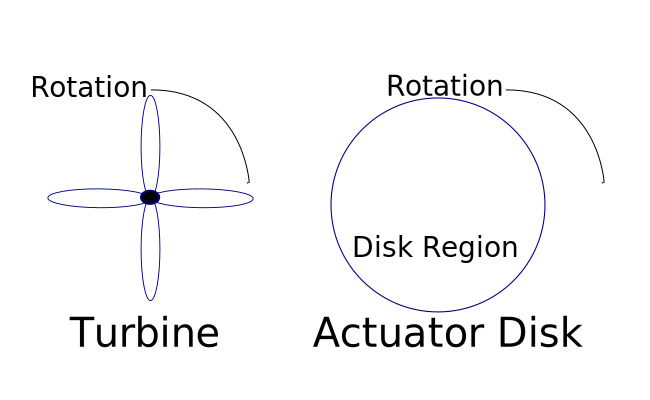
\includegraphics[width =0.95\textwidth]{figs/actuator_disk}
     \caption{The actuator disk model represents a turbine blade
    geometry (shown on the left) as a spinning ``disk'' region (shown
    on the right).}
     \label{fig:actuator_disk}
   \end{figure}

The normal in the blade's velocity direction is,
\begin{equation*}
n_B = \frac{u_B}{||u_B||}. 
\end{equation*}
Where $u_B$ is the blade velocity and is specified. The normal in the
fan vertical direction is typically, $n_v = \left(0,0,1\right)$, 
e.g. pointing ``up''. Then the normal in the radial direction must be, 
\begin{equation*}
n_r = n_B \times n_v. 
\end{equation*}

% The fan-wing-plane bit means that we're only looking at the projection
% of velocity into the plane that's defined by the base velocity and
% vertical direction. 

% (01:03:44 PM) Roy Stogner: The "local relative velocity" means that
% we're taking the velocity not in the reference frame of the domain, but
% in the reference frame of the wing.  So if the base velocity is U_B and
% the air velocity is U, then the local relative velocity is U - U_B. 
% (01:04:25 PM) Roy Stogner: Note that we simplify that equation a tiny
% bit by using the fact that U_B and N_R are perpendicular. 

Then, the fan-wing-plane component (e.g. the plane perpendicular to the 
radius) of local relative velocity is
\begin{equation}
u_p = u - (u\cdot n_r)\cdot n_r - u_B. 
\end{equation}
This is the projection of velocity into the plane that's defined by the
base velocity and vertical direction. 
Now the ``forward velocity'' in the reference frame of the turbine is, 
\begin{equation}
u_{\text{fwd}}= -u_p \cdot n_B
\end{equation}
and the ``upward'' velocity in this frame is, 
\begin{equation}
u_{\text{up}} = u_p \cdot n_v. 
\end{equation}
Finally, we can specify the angle with respect to the fan velocity
direction as, 
\begin{equation}
 \theta_f = \text{atan2}\left(\frac{u_{\text{up}}}{u_{\text{fwd}}}\right)
 %\theta_f = \text{tan}^{-1}\left(\frac{u_{\text{up}}}{u_{\text{fwd}}}\right)
\end{equation}
while the angle with respect to the chord is this with the addition of
the blade angle relative to the fan vertical direction, 
\begin{equation}
 \phi = \theta_f + \beta(r).
\end{equation}

  \begin{figure}[!htb]
    \begin{center}
     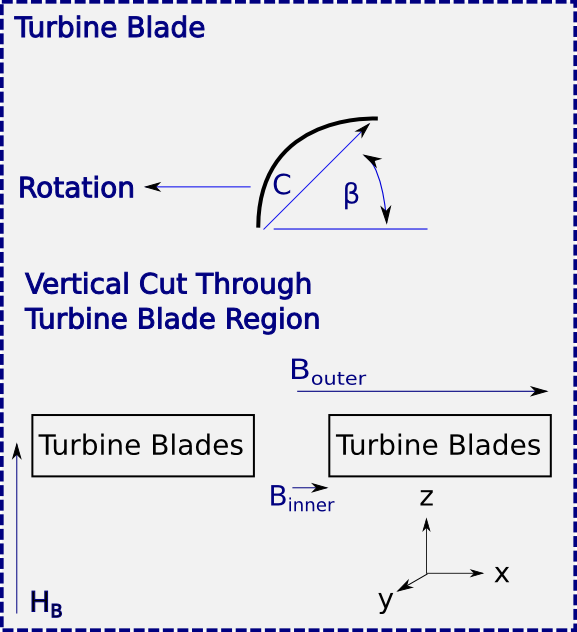
\includegraphics[width = 10 cm]{figs/turbine_image}
     \caption{}
     \label{fig:turbine_image}
    \end{center}
  \end{figure}

In words, the blade angle (or local pitch) is measured from the plane of
rotation to the chord line (i.e., the straight line connecting leading
to trailing edge). These parameters, $\beta$, etc. are visually depicted
in Figure \ref{fig:turbine_image}.  


\subsection{Drag Polar Specification}

Duane says that these were generated with COMSOL.\todo{write to this}

We can now define the lift and drag normals, where the direction
opposing drag is, 
\begin{equation}
n_{\text{drag}} = \frac{u_p}{||u_p||} 
\end{equation}
and the direction opposing lift orthogonal to the drag and the radial direction, 
\begin{equation}
n_{\text{lift}}= n_{\text{drag}} \times n_r. 
\end{equation}

Then, the force on the turbine is, 
\begin{equation}
 \boxed{F = \frac{1}{2}\frac{\rho u_p^2 c}{A}\left(C_l \cdot
					      n_\text{lift} + C_d \cdot n_\text{drag}  \right)}
\end{equation}

Volumetric force is
\begin{equation}
 \boxed{\frac{n F}{2 \pi r t} = \frac{F}{\text{volume}}= \frac{1}{2}\frac{\rho u_p^2 c}{A}\left(C_l \cdot
					      n_\text{lift} + C_d \cdot n_\text{drag}  \right)}
\end{equation}


Where c is the chord length (specified as input), and A is the area,
which is also specified. Now, only the drag polars must be specified in
order to fully determine the force on the blades.

The semi-circular plots are more complicated. Here, we use a high order
polynomial fit to continuously interpolate between drag polars. 

\begin{figure}[!htb]
  \begin{center}
    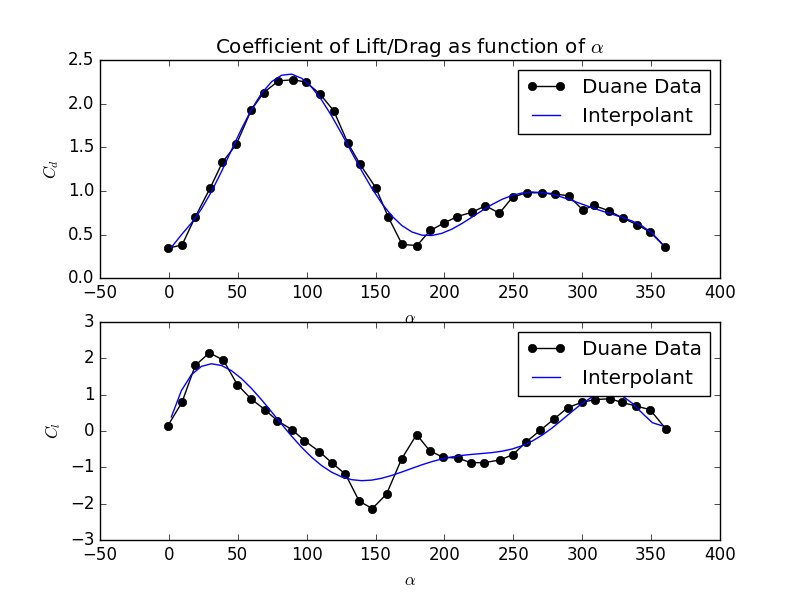
\includegraphics[width = 12 cm]{figs/flat}
    \caption{The flat plate drag polars.} 
    \label{fig:flat_plate_drag}
  \end{center}
\end{figure}

\begin{figure}[!htb]
  \begin{center}
    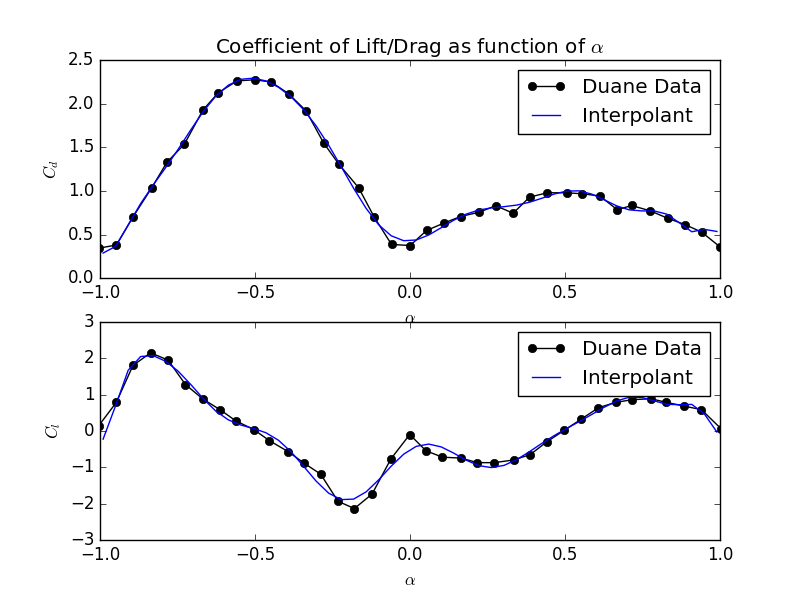
\includegraphics[width = 12 cm]{figs/semi}
    \caption{The semicircle (180 degree) drag polars.} 
    \label{fig:semi_drag}
  \end{center}
\end{figure}

\begin{figure}[!htb]
  \begin{center}
    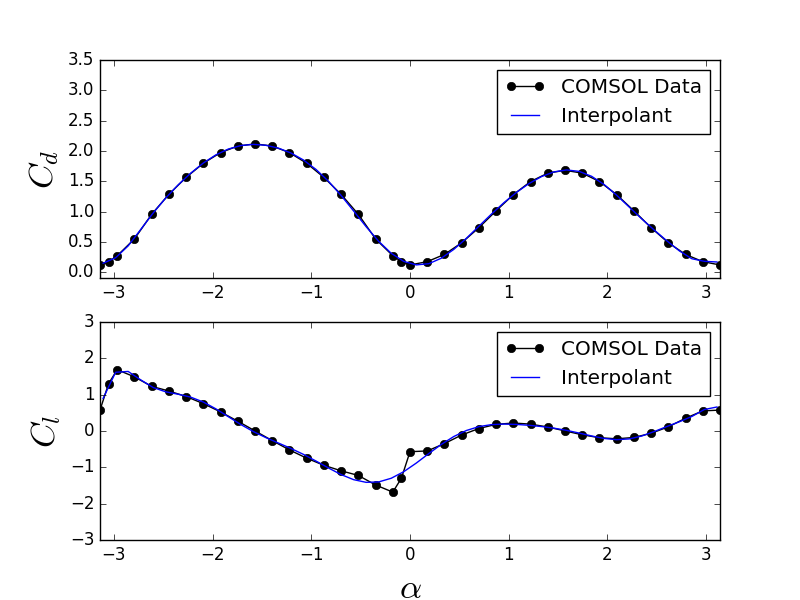
\includegraphics[width = 12 cm]{figs/90}
    \caption{The 90 degree drag polars.} 
    \label{fig:90_drag}
  \end{center}
\end{figure}

what about loads on turbine?\todo{loads?}
%% load was predicted at 20 ft*lbs


\subsection{Wake Loss Model}
\label{subsec:wake_loss_model}

The model's described above do not account for the turbulent wake state,
which in some cases have been shown to be significant for a wind
turbine. The model deficiency results due to the actuator disk
method's dependence on the precision of the lift and drag
coefficients. During the operation of a wind turbine, should the angle
of attack can reach high values (post-stall region), then aerodynamic 
data is not available or inaccurate. 
   
This model inadequacy is commonly fixed with the Glauert Correction. 
Developed in 1926 by Glauert from helicopters rotor blades, this
correction originally was purely based on experimental data. The model
was designed to correct the overall thrust coefficient for high angles
of attack. 

The Glauert correction is a tip loss model.\todo{write me!}

We note that the Glauert correction was developed as a correction to an
entire rotor disk; the original researchers did not intend it to be
applied to a rotor annulus. However, because of a limited amount  of
experimental data, an alternative model does not exist.  

Various researchers\cite{?} (Wilson and Patton  1978) have suggested
various other corrections to actuator-disk theory. These corrections
include (among others) accounting for blade thickness on local angle of
attack, cascade width for high solidity turbines, and spanwise gaps for
partial span pitch control. The impact of these missing physics can be
significant, for instance, blade thickness and effects can be  
aerodynamically significant near the rotor hub and may affect the
in-plane forces on the rotor\cite{?}. Nevertheless, these corrections
are not treated in the simulations presented in this document. 

\section{Solid Surface Representation}
\label{subsec:solid_surface}

In addition to vanes, the SoV device includes impermeable surfaces
such as the wind break (``cone'') on the top of the facility. As with
the turning vanes, this is represented without explicitly meshing the
surface nor imposing  a boundary condition at the surface. This allows
rapid exploration of configurations  with different solid surfaces to
control and manipulate the fluid flow. These solid surfaces are
represented by a body force acting in a region surrounding the wall. 
A body force normal to the surface is defined in this region so
that it will drive the normal velocity to zero, resulting in the flow
moving only parallel to the virtual surface. 
The body force is defined as in Equation
\ref{eqn:body_force}; however, the length scale $\ell_v$ is specified to
be identical to the width of the surface being represented. This is
typically the width of two or three grid cells. While the actual surface we are
emulating is thinner than this, the numerical method has difficulty
converging for surfaces smaller than the grid size.  

Forcing models designed to mimic a surface
are not unique to this project, and the current formulation is
 closely related to (among others)
``immersed boundary methods'' as used by various other
researchers\cite{doi:10.1146/annurev.fluid.37.061903.175743}. 
This approach is unique in its use of Babuska's penalty treatment of
constraints\cite{1973fempen,ZAMM:ZAMM19880680925} to enforce the
behavior at the boundary. This method was selected because it is easily
imposed in the FEM context, and the method has been explored in detail
in the literature.\todo{add more discussion of healing length implications here}
%Typically, the enforcement occurs along a domain
%boundary, but in this work it is used in the interior, 
%and is not imposed as a mathematical constraint but rather as a modeling 
%approach. 

% We add a penalty term to the weak
% form of the Navier-Stokes momentum equation described in the subsequent
% section %\ref{eq:ns_weak} 
% that has the form, 
% \begin{equation}
% P_\epsilon = \int_\Omega ({\bf f_v} \cdot v) \, dx
% \end{equation}
% where ${\bf f_v}$ is as described in equation \ref{eqn:body_force}. 
%% As the system is formulated as a variational problem that seeks to
%% minimize the test function $v$, any velocity that is not aligned with
%% the vane normal will incur a penalty versus one that does. Note that unlike
%% some penalty methods, this does not automatically satisfy
%% continuity. Rather, the velocity field remains divergence free through a
%% separately enforced constraint.  

\section{Separation Model}

In the presence of wind, it was found that there was a significant flow
out through the vanes in the back of the device. This was obviously
inconsistent with the findings of our colleagues in the field, who
observed no outflows out of the back of the device. Moreover, this resulted
in large inconsistencies between our predictions and the field results,
almost certainly because of the kinetic and thermal energy that our vane
representation was permitting to leave out the back of the device.  

This exposed a weakness of the turning vane representation outlined
previously. When the flow entered the virtual vane forcing region it was
always turned to align with the vane angle, even when the forcing was in
the opposite direction of the present velocity.
This is in contrast to the physical situation, in which we
expect the flow to continue along an averaged streamline separating from the 
trailing edges of the vanes, instead of turning around it. 
The averaged streamline will continue past the trailing edge of the vane
due to the separation of the boundary layer off the edge surface. An
image depicting these two cases in shown in Figure \ref{fig:sep_model}.  

\begin{figure}[!htb]
  \begin{center}
    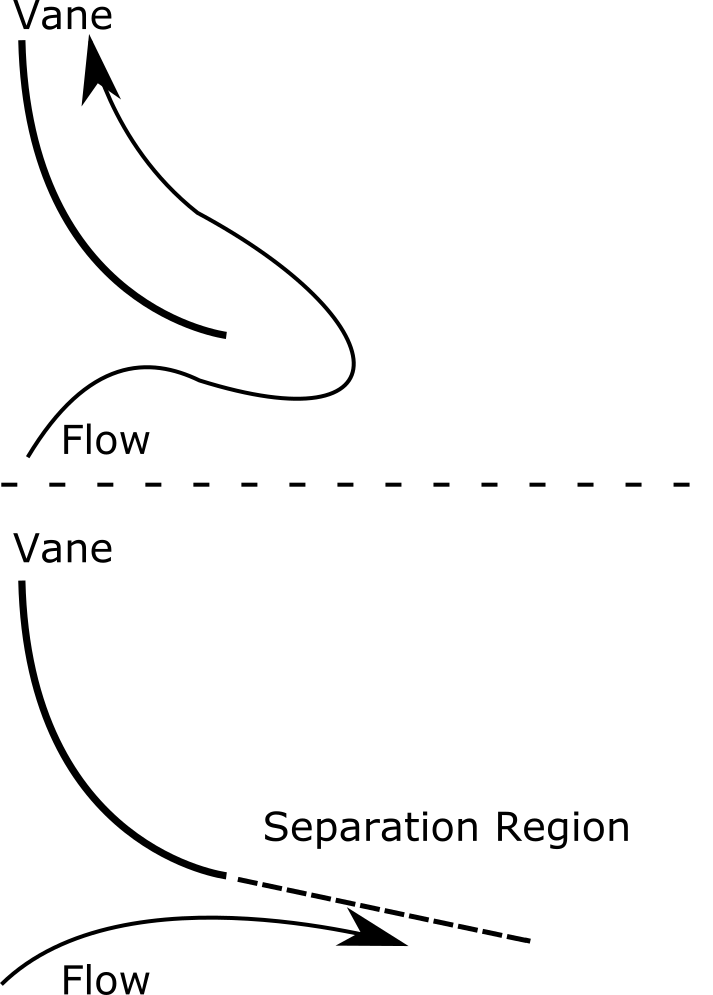
\includegraphics[width = 6 cm]{figs/sep_model}
    \caption{Schematic depicting the separation model that extends past
   the trailing edge of the vanes. In the top case, the flow entering
   the virtual vane region is forced to align with the vane angle despite
   this resulting in a reversal of the flow direction. This is a
   consequence of the forcing function acting on the fluid to ensure the
   velocity vector aligns with the vane. 
   The second case depicts the separation
   model, where the flow under certain conditions is not forced and
   continues to move tangent to the vanes due to 
   the separation of the boundary layer off the trailing edge.} 
    \label{fig:sep_model}
  \end{center}
\end{figure}

Let $\bf n^v$ be the normal vector to the vanes,
and $\bf n^r$ the normal vector pointing out of the vane
region\footnote{\normalsize The superscripts ``v'' and ``r'' stand for
vane and radial, respectively.}.  
Then, $\bf t^v$ is the tangential vector to the vanes pointing out of
the vane region and is defined as,

%\begin{equation}
% \bf t^v = \left( {\bf n^v_y},{\bf -n_x^v} \right) \text{sign}\left[
%	    \left( {\bf n^v_y},{\bf -n_x^v} \right) \cdot {\bf n^r} \right].
%\end{equation}
\begin{equation}
 \bf t^v = \left( {\bf n^{v^\perp}} \right) \text{sign}\left(
	    {\bf n^{v^\perp}} \cdot {\bf n^r} \right).
\end{equation}
Here, ${\bf n^{v^\perp}}$ is the vector perpendicular to the normal
vector of the vanes, which is simply, 
\begin{equation*}
 {\bf n^{v^\perp}} = \left[ \begin{array}{c}
n_x\\
n_y\\
\end{array}\right]^{\perp} = 
 \left[ \begin{array}{c}
  -n_y\\
  n_x\\
	\end{array}\right].
\end{equation*}

%
% example of an algorithm
%

\begin{center}
 \begin{algorithm}
  \caption{The crude separation model. This model identifies if the flow
  is coming into or out of the vane region, and if the velocity vector
  is in the same direction as the tangent line of the vanes. In the case
  of the ``special forcing'' the flow is forced as if it was
  impacting a solid surface. In the
  algorithm below, $r_0$ is the max radius of vanes, $r_i$ the minimum
  radius of vanes, and $\delta$ is the width of the separation region.}
  \label{alg:sep}
  \begin{algorithmic}
   \IF{($r_0 > r > r_i$)} 
   \IF{$(r_0 - r) < \delta$ \textbf{or} $((r - r_i) < \delta)$}
   \STATE ${\bf n^r} = {\bf r}/|r|$
   \IF{$(r - r_i) < \delta$} 
   \STATE ${\bf n^r} = -{\bf n^r}$
   \ENDIF
   \STATE  $\bf t^v = \left( {\bf n^{v^\perp}} \right) \text{sign}\left(
  	    {\bf n^{v^\perp}} \cdot {\bf n^r} \right)$
   \IF{$v \cdot t^v > 0$ \textbf{and} $v \cdot n^r < 0 $}
   \STATE ${\bf n}({\bf x}) = \hat r$ \quad (Special Forcing)
   \ELSE
   \STATE  ${\bf n}({\bf x}) = \sin \left(\phi(r) \right) \hat{{\bf r}}+ \cos
  \left(\phi(r) \right) \hat{{\bf \theta}} $
  \quad (Normal Forcing)
   \ENDIF
   \ELSE
   \STATE ${\bf n}({\bf x}) = \sin \left(\phi(r) \right) \hat{{\bf r}}+ \cos
  \left(\phi(r) \right) \hat{{\bf \theta}} $
  \quad (Normal Forcing)
   \ENDIF
   \ENDIF
  \end{algorithmic}
 \end{algorithm}
\end{center}


The forcing is modified when the velocity vector of the local flow, $\bf
u$ is pointing in to the forcing region: ${\bf u} \cdot {\bf n^r} < 0$, and
when the velocity vector is in the same direction as the tangent line to
the vanes: ${\bf u} \cdot {\bf t^v} > 0 $. In these instances, the
forcing acts as if there was a rigid surface past the vane edge, and
gives the appearance of a special ``no-penetration'' condition for the
velocity for these cases. The pseudo-code for this procedure is shown in
Algorithm~\ref{alg:sep}.

The addition of this simple separation model significantly reduced the
flow that penetrated the back of the vanes, and produces results
consistent with the observations provided by our experimental
colleagues.  

\section{Effect of Surface Roughness}

%%
%% this does not describe the phenomena being modeled or the precise
%% model -- rewrite
%%
%%
%% this does not say enough about the surface roughness
%% motivate that and explain how it is used, than show your estimate 
%% to argue it is small
%%

Surface roughness effects have been shown to play a role in the
formation of dust devils and related atmospheric
phenomena\cite{oke1987boundary}. For the flat and sandy regions we are
simulating, the impact is expected to be a small velocity perturbation 
in the vertical direction. This is modeled as a volumetric 
forcing in a narrow region above the surface,
\begin{equation}
 F^{'''}_{z_0} = \frac{1}{2}\rho V_z^2/z_{0}, 
\end{equation}
where $z_{0}$ is the roughness height. We ensure that the energy
introduced into the flow is a small fraction of total flow energy by comparing
this with the energy flux through the top of the vanes. The total energy
added is measured as,  
\begin{equation}
 E_{\text{injected}} = \int_0^{2\pi} \int_0^R \int_0^{z_0} F^{'''}_{z_0}
  dz dr d\theta.  
\end{equation}
R is the outer diameter of the vanes. 
The value of $E_{\text{injected}}$ is typically a few percent of the
total kinetic energy flux measured through the top of the
vanes.\todo{expand this section}

%This general forcing provides additional capabilities including the
%ability to investigate engineering greater surface roughness or
%structures that could provide greater ``kick-up'' of the thin thermal
%layer near the surface into the flowing regime. It can also support more
%general turning configurations than the virtual vanes outlined above. 

\section{Turning Vane Drag}

yar\todo{write me}

\section{Simulation Geometry and Boundary Conditions}
\label{sec:bc}

In this project, two principle modeling regimes are considered. 
One is the ``thermal-only'' scenario, in which there are no ambient
velocities and there is an imposed elevated temperature on the ground.  
In the other, there are also ambient winds that contribute to the SoV energy
(``wind'' cases). 
The computational domain and boundary conditions for these 
two scenarios are described below.

\textbf{Computational Domain} 

All simulations are performed in a cuboid domain, with six
faces.  The domain is denoted $\Omega \subset \mathbb{R}^3$. 
The domain extents are scaled by the system diameter, D, created by the
outer vane radius. The extents are defined in terms of $\{L_x,L_y,L_z\}$ indicating the 
streamwise, spanwise and vertical directions, respectively. 
For both simulation regimes, sensitivity analyses 
were performed to ensure that the results were not sensitive 
to the domain extents. For the thermal-only case, for which $L_x = L_y$,
the system 
extents $L_x/D$ and $L_y/D$ are chosen to be 3. The height ($L_z/D$) is
three times the system diameter, which is typically nearly equal to the
height of the vanes. This defines the thermal-only domain $\Omega_T$, 
as $\Omega_T = \left[-L_x,L_x \right] \times \left[-L_y,L_y \right]
\times \left[0,L_z \right]$.   

For the wind cases, the streamwise extent is no longer equal to
the spanwise length, $L_y$. In these cases, the domain length extends
two diameters in front of the vanes and three behind. The
spanwise direction is symmetric and extends two diameters in each direction 
from the center ($L_y/D = 2$). The height is identical to the
thermal-only case, at three system diameters ($L_z/D = 3$). Thus, the
wind domain is defined as $\Omega_W = \left[-2D,3D \right] \times
\left[-L_y,L_y \right] \times \left[0,L_z \right]$.   

The boundary for the thermal only case is decomposed as,
$\partial \Omega_T = \Gamma_G \bigcup \Gamma_T \bigcup \Gamma_P $. 
$\Gamma_G$ is the boundary along the ``Ground'', $\Gamma_T$
the ``Top'' boundary, and $\Gamma_P$ the four periodic ``Sides''. A 3d
diagram labeling these boundaries is shown in
Figure~\ref{fig:thermal3d}. For this case study (no mean wind),
periodic boundary conditions are used on the four sides , with a modified 
``inflow-outflow'' Neumann condition\cite{gunzburger1989finite} on the
top boundary. On the ground, a ``no-slip'' velocity boundary condition is
imposed, and a Dirichlet condition uniformly fixes
the temperature of the surface. 
Each of the $\Gamma$ boundary terms are defined in the paragraphs below. 
Note that a finite thickness ``Sponge Layer'' is
indicated on the figure along the top boundary and is defined below. 

\begin{figure}[!htb]
  \begin{center}
    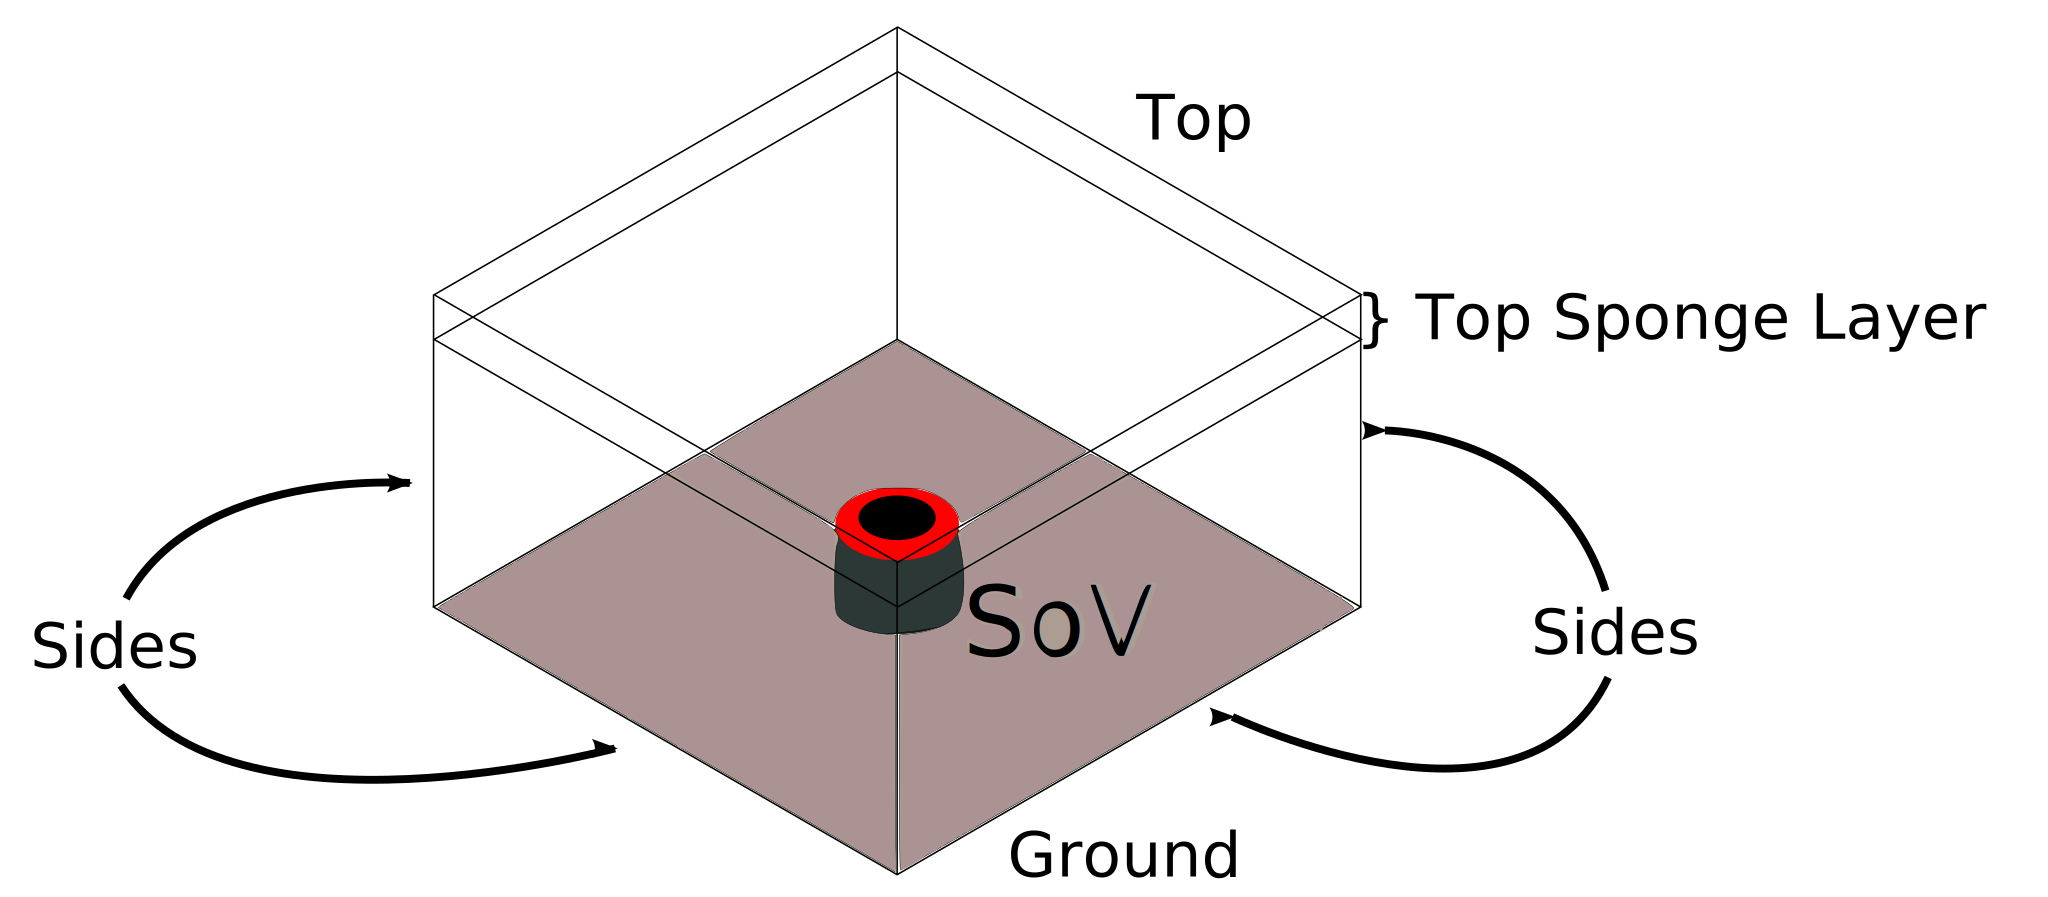
\includegraphics[width=14cm]{figs/thermal_only_3d}
    \caption{Domain for the thermal-only
   scenario. The diagram scale is representative of typical cases. Note
   the SoV apparatus in the center, which provides perspective on the
   extent of the domain with respect to the turning vane diameter. The
   ground, sides and top boundaries are labeled with the discussion the
   precise boundary conditions on each provided in
   section~\ref{sec:bc}. Notice also the finite thickness, high
   viscosity ``sponge layer'' at the top of the domain.} 
    \label{fig:thermal3d}
  \end{center}
\end{figure}

The boundary for the wind cases is decomposed as,
$\partial \Omega_W = \Gamma_G \bigcup \Gamma_T \bigcup \Gamma_O \bigcup
\Gamma_I \bigcup \Gamma_S $.  
Where $\Gamma_G$ is the boundary along the ``Ground'',
$\Gamma_T$ the ``Top'' boundary, $\Gamma_S$ the two ``Sides'',
$\Gamma_I$ the inflow boundary, and $\Gamma_O$ the ``Outflow''  
boundary.
The ``wind'' simulation domain is diagrammed in
Figure~\ref{fig:wind3d}, with the boundaries labeled. 
For this particular study (a heated ground with 
an ambient wind), the wind case has a proscribed inlet boundary layer
along the upstream streamwise face ($\Gamma_I$) for both the temperature
and the velocity. The ``Ground'' boundary is identical to
the thermal-only case. The ``Sides'', ``Outflow'' and ``Top'' are all
set to modified Neumann boundary conditions. Note that ``Sponge Layers''
are used on both the back boundary and the top. 

\begin{figure}[!htb]
  \begin{center}
   \includegraphics[width=14 cm]{figs/wind_3d}
    \caption{Domain for the wind and thermal scenario. The diagram scale
   is representative of typical cases. Note the SoV apparatus which
   provides perspective on the extent of the domain with respect to the
   turning vane diameter. The ground, sides, inflow, back and top
   boundaries are labeled with the discussion the precise boundary
   conditions on each provided in section~\ref{sec:bc}. Notice also the
   finite thickness, high viscosity ``sponge layer'' at the top and back
   of the domain.}   
    \label{fig:wind3d}
  \end{center}
\end{figure}

\textbf{Ground Boundary Conditions, $\Gamma_G$} 

For both the wind and thermal-only cases the ground has a fixed
temperature and no-slip velocity boundary conditions. This boundary 
($\Gamma_G$) is modeled with a Dirichlet boundary condition, 
\begin{align}
 {\bf u} &= 0 \quad \text{ on } \Gamma_G \\
 T &= T_g.
\end{align}
Where $\Gamma_G = \{(x,y,0) \subset \partial \Omega \} $. 

%
% http://fenicsproject.org/documentation/dolfin/dev/python/demo/documented/periodic/python/documentation.html 
%
%
\textbf{Periodic Boundary Condition, $\Gamma_P$} 

A periodic boundary condition is used in the thermal only cases, 
along the streamwise and spanwise boundary faces 
(denoted $\Gamma_{P,x}$ and $\Gamma_{P,y}$, respectively). In these
cases the state variables  
are contrained to have the same value on the opposite faces of the domain, 
for instance in the streamwise direction the boundary conditions are, 
\begin{align}
 {\bf u}(-L_x,y,z) &= {\bf u}(L_x,y,z) \quad \text{ on } \Gamma_{P,x} \\
 T(-L_x,y,z) &= T(L_x,y,z)
\end{align}
and in the spanwise direction,
\begin{align}
 {\bf u}(x,-L_y,z) &= {\bf u}(x,L_y,z) \quad \text{ on } \Gamma_{P,y} \\
 T(x,-L_y,z) &= T(x,L_y,z). 
\end{align}
Where $\Gamma_{P,x} = \{(-L_x,y,z) \bigcup (L_x,y,z) \subset \partial
\Omega \}$  
and $\Gamma_{P,y} = \{(x,-L_y,z) \bigcup (x,L_y,z) \subset \partial
\Omega \}$. 

\textbf{Inflow Boundary Condition, $\Gamma_I$} 

On the inflow boundary $(\Gamma_I$), dirichlet conditions are used for both
velocity and temperature. The boundary-normal, or streamwise component 
is a function of the surface normal coordinate (z), representing a boundary 
layer below a uniform velocity, U.
The common 7th power model of a turbulent boundary layer is used,   
\begin{equation*}
  u_{\text{in}}(z) = U \text{ min }\left(\left(\frac{z}{\delta}\right)^7,1\right)
  \label{eq:bl_u}
\end{equation*}
where $\delta$, the boundary layer thickness, is set based on data
measured by our experimental partners in the field. 
The thermal boundary layer is assumed to have a similar boundary layer,
but, as observed in real atmospheric flows, there remains a vertical
temperature gradient outside the thin boundary layer. Based on
results in the literature a $2/3$ Kelvin per meter gradient is 
imposed\cite{Blocken2007238}. The thermal inflow is then  
\begin{equation*}
  T_{\text{in}}(z) = \Delta T \left(1- \text{ min
			}\left(\left(\frac{z}{\delta}\right)^7,1\right)\right)
  + T_0 - 2z/3.  
  \label{eq:bl_t}
\end{equation*}
% 335+18*tanh(-z/0.1)-z*2/3
The inflow boundary is at the surface $x=-L_x$.\todo{add image of how
inflow boundary layer profile is roughly correct}

\textbf{Mixed inflow/outflow Boundary Conditions on $\Gamma_T$,
$\Gamma_S$ and $\Gamma_B$}  

At outflow boundaries, a homogeneous ``do nothing'' Neumann condition is
appropriate\cite{Rannacher2000}, 
\begin{align}
  \frac{\partial u}{\partial n}\bigg|_{\Gamma_T} = 0 \\
  \frac{\partial T}{\partial n}\bigg|_{\Gamma_T} = 0
\end{align}
However, for the cases in this study, a modified Neumann condition is
necessary due to the possibility that there will be an inflow on these
boundaries. 
For example, in the region above the vanes, the concentrated hot plume is
lifted by buoyancy upward and out of the simulation domain. However, the
radial inflow towards the apparatus is drawn in by large scale
convection cells larger than the system diameter. Thus, our boundary
conditions must permit inflow along the areas above and external to the
vanes, while simultaneously permitting outflow in the area above the vanes. 

% Roy Stogner: Okay, so this DDN is basically no-traction when there's 
% outflow and Tn=v when there's inflow?  We have no-traction for v*n, 
% no-traction for anything else when there's outflow, and Dirichlet
% v.cross.n = 0 when there's inflow. 

To accomplish this, the boundary condition is,
\begin{align}
  \frac{\partial u_n}{\partial n}\bigg|_{\Gamma_T} = 0 \\
  \text{if } (w<0) \text{ then}& \begin{cases}
    u_t = 0,\\
    T = T_{\text{in}}
  \end{cases} \\
  \text{ else}& \begin{cases}
    \frac{\partial u_t}{\partial n}\bigg|_{\Gamma_T} = 0, \\  
    \frac{\partial T}{\partial n}\bigg|_{\Gamma_T} = 0
  \end{cases}
\end{align}

where $u_n$ and $u_t$ are normal and tangential components of the velocity, 
respectively. This boundary condition is applied on the top boundary
$\Gamma_T$ ($z=L_z$) and downstream side boundary  $\Gamma_B$ in the wind case.

\textbf{Sponge Layer} 

Finally, a finite thickness ``sponge layer'' is used in the region adjacent 
to the mixed inflow/outflow boundaries $\Gamma_T$ and $\Gamma_B$.
This layer artificially increases the momentum diffusivity by
up to a factor of ten times the nominal value. This was designed to stabilize
the modified Neumann boundary conditions which can exhibit an instability
when there is a compact jet of fluid leaving the domain. 
These small outflows would create small high velocity inflows, and the
feedback loop would result in instabilities and numerical
blow-up. Mindful of the fact that the character of solution not
important in this region, and that our physical interest remains focused
on the region inside and in immediate proximity to the vanes, we
introduced a higher diffusivity ``sponge'' region that would diffuse the
high velocity exiting jets sufficiently to prevent numerically
un-physical behavior. No results are quoted from this ``sacrificial''
region, as it is not considered physically meaningful.

These regions are referred to by many names in the
literature\cite{doi:10.1146/annurev.fluid.36.050802.121930}, such as
absorbing layers, fringe regions, buffer zones, sponges,
etc.\todo{expand this? how thick did it need to be?}
